
%
% raspberry p3 spec: https://www.raspberrypi.org/magpi/raspberry-pi-3-specs-benchmarks/

\section{Embedded Computing Platform Comparison}\label{sec:comparison}

In this section, we compare three computing platforms---the Raspberry
Pi 3, the Intel UP~\footnote{http://www.up-board.org/up/} and NVIDIA
Jetson
TX2~\footnote{http://www.nvidia.com/object/embedded-systems-dev-kits-modules.html}---from
the point of view of supporting vision-based end-to-end deep learning
based autonomous vehicles. 
Table~\ref{tbl:platforms} shows architectural features of the three
platforms~\footnote{Note that the GPUs of the Raspberry Pi 3 and Intel
  Up are not used in evaluation due to lack of software (TensorFlow)
support. Also, the two Denvor cores in Tegra TX2 are not used in
evaluation due to TensorFlow issues.}.
  
Our basic approach is to use the same DeepPicar software, and repeat
the experiments in Section~\ref{sec:evaluation} on each hardware
platform and compare the results. 
For Tegra TX2, we have two different system configurations,
which differ in whether TensorFlow is configured to use its GPU or
only the CPU cores. Thus, the total four system configurations are
compared.

\begin{figure}[h]
  \centering
  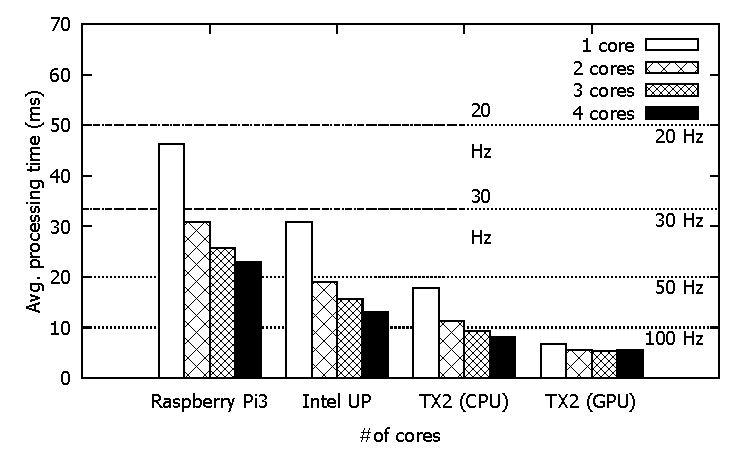
\includegraphics[width=.5\textwidth]{figs/compare_core}
  \caption{Inferencing time across platforms based on number of cores 
used.}
  \label{fig:sys_core}
\end{figure}

Figure~\ref{fig:sys_core} shows the average control loop completion
timing as a function of the number of CPU cores on each of the four
system configurations.
It was found that the both the Tegra TX2 
and the Intel UP Board performed better than the Raspberry Pi 3 in 
all experiments. On average, the UP was able to perform inferencing 
operations, at least, twice as fast as the Raspberry Pi 3. The 
difference was even greater with the TX2, as control loops, in the 
worst case, were 3x faster using only the CPU and 10x quicker when 
using the GPU. As a result, they were all able to satisfy the 50 ms 
WCET by a very clear margin (in the worst case, the UP Board would 
still meet it by $\sim$20 ms), and, thus, demonstrates that they are 
more capable of autonomous driving than the Raspberry Pi 3.

The UP Board and TX2 also performed better in the multimodel tests, 
as is shown in Figure~\ref{fig:sys_model}. Once again, they were able 
to complete control loops in a fraction of the time when compared to 
the Pi. Furthermore, both of the platforms satisfied the 50 ms WCET 
in all experiments, while the Raspberry Pi 3 was unable to do so. As 
such, the UP Board and TX2 display greater potential for the 
simultaneous execution of multiple models during self-driving 
operation, while the Raspberry Pi 3 would struggle to do so.

\begin{figure}[h]
  \centering
  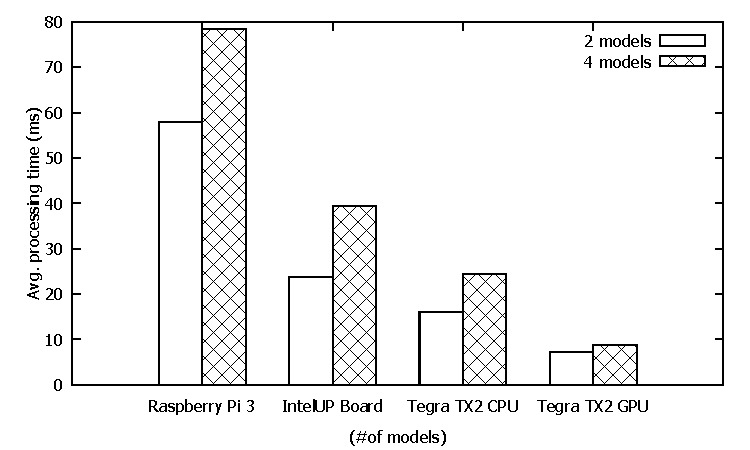
\includegraphics[width=.5\textwidth]{figs/compare_model}
  \caption{Inferencing time across platforms based on number of 
models run concurrently.}
  \label{fig:sys_model}
\end{figure}

Finally, we examined if the performance of the Intel UP Board and 
Tegra TX2 would be affected by the addition of the synthetic 
benchmarks. As summarized in Figure~\ref{fig;sys_bench}, the both 
experienced a change in their inferencing times, but the increases 
were not as drastic as is seen by the Raspberry Pi 3. in the worst 
case, both the UP Board and TX2 (CPU only and GPU) produced times 
that were over two times as large, whereas the Raspberry Pi 3 output 
times that were around 10 times greater. The Intel UP Board was 
successful in completing inferencing operations in under 50 ms when 
benchmarks were run on a maximum of 2 cores, and the TX2 was 
successful in all experiments irrespective of the computing resources 
utilized. Comparetively, both performed better than the Raspberry Pi 
3 which failed to meet its deadlines when any benchmark was 
introduced. As such, it can be concluded that the Intel UP Board 
would be more capable of running computationally heavy processes 
during autonomous driving, and that the Pi wouldn't be able to do the 
same.

\begin{figure}[h]
  \centering
  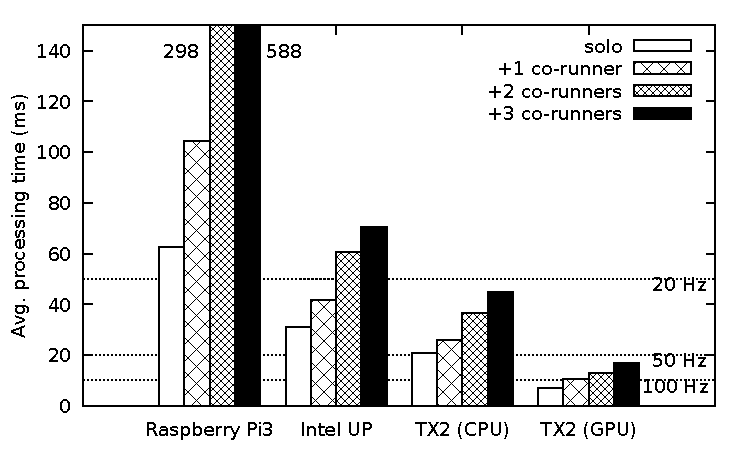
\includegraphics[width=.5\textwidth]{figs/compare_benchmark}
  \caption{Inferencing time across platforms based on number of cores 
used.}
  \label{fig:sys_bench}
\end{figure} 

In the comparison of the real-time capabilities of three embedded 
computing platforms, we found that the Raspberry Pi 3 performed the 
worst. When compared to the Intel UP Board and the NVIDIA Tegra TX2, 
control loops on the Pi were shown to take noticably longer to 
complete, regardless of the number of cores utilized or the number of 
neural network models run simultaneoulsy. The difference was even 
more noticeable in the the addition of computationally heavy 
synthetic benchmarks that had a much more dire effect on the Pi. In 
the worst case, an average control loop on the Pi took an abnormally 
long amount of time to finish. Compared to the TX2 with GPU support, 
those times were 34.8X times greater. From this, we find that the UP 
Board and Tegra TX2 are superior platforms for real-time CNN 
operations. However, due to the Pi's ability to satisfy the 50 ms 
WCET in some experiments, we conclude that the Raspberry Pi 3 is 
feasible for autonomous research.



